% Venue-neutral research review; NOT SUBMITTED. Author fields intentionally blank.
% Standard article class; retained publisher files are not compiled.
\documentclass[11pt,a4paper]{article}
\usepackage[margin=27mm]{geometry}
\usepackage[T1]{fontenc}
\usepackage{mathptmx}
\usepackage[numbers,sort&compress]{natbib}
\usepackage{url}
\providecommand{\hypersetup}[1]{}
\providecommand{\hypertarget}[2]{#2}
\providecommand{\hyperlink}[2]{#2}
\providecommand{\href}[2]{#2}
\providecommand{\texorpdfstring}[2]{#1}
\usepackage{graphicx,amsmath,amssymb,booktabs,array,textcomp}
\hypersetup{colorlinks=true,linkcolor=black,citecolor=black,urlcolor=blue,pdfauthor={}}
\setlength{\emergencystretch}{3em}
\newlength{\JournalTableWidth}
\providecommand{\tightlist}{\setlength{\itemsep}{0pt}\setlength{\parskip}{0pt}}
\providecommand{\passthrough}[1]{#1}
\providecommand{\pandocbounded}[1]{#1}
\raggedbottom
\begin{document}
\title{Correctable Category Priors for Budget-Constrained Active Observation}
% Author name, affiliation, email and ORCID: deliberately not supplied.
% \author*[1]{\fnm{} \sur{}}\email{}
% \affil*[1]{\orgdiv{},\orgname{},\orgaddress{\city{},\country{}}}
\author{}
\date{Anonymous research draft, 8 November 2026}
\maketitle
\begin{abstract}
Robotic observation must allocate a limited motion budget between discovering unknown space and recovering incompletely measured surfaces. Category cues can predict useful viewing directions, but their value depends on whether they change an affordable route and remain correctable by acquired geometry. We study this mechanism using bounded geometric evidence, diagnostic lookahead and return-feasible planning, while reconstructing surfaces only from measured depth. A controlled two-template study uses exact poses, public pose graphs and synthetic category cues. Against a matched active geometric control, four reference configuration pairs yield two improvements and two ties, increasing mean coverage--surface quality by 6.16\% at unchanged planar coverage. Two changed-background layouts yield one improvement and three ties, with a 2.98\% mean gain. A 128-attempt extension retains 32 low-budget planning failures and a 0.70\% larger-budget reversal. A separate joint-exploration variant starts from actual simulated observations rather than a supplied complete graph. Its 24 deterministic trajectories in one scene context show coverage--surface tradeoffs and a late surface gain, without faster early semantic coverage; a two-room geometric-weight control reproduces the semantic trajectory. A prospectively fixed additional synthetic parent yields a surface gain, while saved-state weight checks leave category-specific attribution unresolved. Physical pilots retain two incomplete S returns alongside a completed 24-action loop whose map may already have drifted. These findings identify conditional observation-allocation effects; general exploration efficiency, natural-semantic benefit and physical reconstruction accuracy remain unverified.
\end{abstract}
\noindent\textbf{Keywords:} unknown-space exploration, active observation, category priors, geometric feedback, budget-constrained reconstruction

\noindent\textit{Anonymous manuscript draft; not submitted.}

\hypertarget{introduction}{%
\section{Introduction}\label{introduction}}

Joint unknown-space exploration and surface observation seek sensing routes that discover accessible space and recover equipment surfaces while preserving enough resources to return to the start. Industrial applications motivate the use of robotic systems \cite{ref9}. We consider maintaining spatial records after workspace reconfiguration as a motivating task. For this task, broad floor coverage can coexist with missing equipment faces: a robot may observe a corridor while leaving a recessed opening or the far side of a cabinet unseen. Useful observation directions therefore matter alongside the amount of space traversed.

The central decision is which viewing direction to choose before acquired geometry resolves the equipment configuration. Active mapping and reconstruction planning can seek diagnostic viewpoints \cite{ref10}, but obtaining that information consumes part of the same budget needed to inspect surfaces and return. A category associated with a particular opening or service side can supply an earlier preference. The benefit depends on whether that preference changes an affordable, consequential route; an incorrect cue must remain revisable when geometric evidence contradicts it.

We study a category-conditioned observation policy that connects configuration belief, diagnostic lookahead, and return-constrained execution. A finite category prior weights two public configuration hypotheses. The planner evaluates future exposure and a possible diagnostic observation, executes one feasible action, and replans after bounded residual evidence updates the belief. Acquired depth is fused separately into the measured reconstruction. Thus, the same configuration hypotheses guide where to sense without supplying unobserved surfaces to the reconstructed output.

This formulation makes the value of a category cue testable against an active geometric alternative. Both policies retain the same graph, templates, diagnostic opportunities, action budget, and reconstruction backend; only the category support differs. A two-configuration analysis relates the value of immediate route selection to the cost and reliability of geometric diagnosis. Recorded beliefs and actions then connect that decision-level account to measured endpoint quality, separating a changed internal score from an actual change in observation allocation.

We distinguish a controlled category-information mechanism from the broader unknown-exploration objective. The supplied-graph simulation yields two improvements and two ties across four reference configuration pairs, increasing mean joint coverage--surface quality by 6.16\% at unchanged coverage. Two changed-background layouts yield one improvement and three ties, with a 2.98\% mean gain. The 128-attempt extension retains 32 planning failures and a 0.70\% larger-budget reversal. A separate joint-exploration variant builds its planning state from acquired sensor observations. Its related simulation conditions show late surface-allocation effects and baseline tradeoffs, while physical pilots include both completed loops and a failed return. These evidence levels do not establish faster unknown-space coverage, natural-semantic benefit or physical reconstruction accuracy.

The contributions are:

\begin{enumerate}
\def\labelenumi{\arabic{enumi}.}
\tightlist
\item
  A task-specific observation formulation couples correctable category support, diagnostic lookahead, and a return budget, with an explicit separation between public planning hypotheses and measured reconstruction.
\item
  A two-configuration decision analysis and recorded belief--action traces explain when an early cue changes a useful route and when geometric diagnosis can remove its advantage.
\item
  A matched evaluation connects information changes to complete routes and measured surfaces, preserving ties, reversals and feasibility failures. Separate unknown-exploration and physical diagnostics test the limits of transfer without conflating their policy versions or experimental units.
\end{enumerate}

\hypertarget{related-work}{%
\section{Related Work}\label{related-work}}

\hypertarget{active-mapping-and-hierarchical-exploration}{%
\subsection{Active mapping and hierarchical exploration}\label{active-mapping-and-hierarchical-exploration}}

Active mapping chooses motion to improve an environmental representation while accounting for state estimation \cite{ref10}. TARE coordinates local and global exploration at different resolutions \cite{ref5}, and Active Neural SLAM uses a learned hierarchy to separate strategic decisions from execution \cite{ref1}. We use this separation to study observation allocation under a return budget. Exact poses and a shared safe graph hold navigation resources fixed so that the controlled comparison concerns the value of category information.

\hypertarget{reconstruction-driven-view-planning}{%
\subsection{Reconstruction-driven view planning}\label{reconstruction-driven-view-planning}}

Reconstruction-driven view planning seeks observations that improve surface recovery. GenNBV learns a next-best-view policy from geometric, semantic, and action representations in a five-dimensional viewpoint space \cite{ref6}. Our planner evaluates explicit configuration hypotheses on a discrete ground-motion graph. It uses predicted exposure to rank observations, while the measured output is reconstructed using Open3D \cite{ref4} and volumetric range integration \cite{ref11}. This design enables a direct comparison of early category information under common motion and fusion resources; generalization to the broader view-planning settings studied by learned policies remains untested.

\hypertarget{semantic-information-for-observation-planning}{%
\subsection{Semantic information for observation planning}\label{semantic-information-for-observation-planning}}

Semantic inspection links target meaning with sensing requirements. SWAP combines exploration, semantic completion, and surface inspection \cite{ref2}; predictive inspection planning uses repeated semantic scene-graph structures to anticipate unseen targets \cite{ref7}. VISTA couples task relevance with directional coverage in online semantic Gaussian mapping \cite{ref3}, and ActiveSGM combines semantic and geometric uncertainty to estimate observation informativeness \cite{ref8}. Here, category information weights alternative hidden configurations of one facility, and contrary acquired geometry can revise those weights before the next return-feasible route is selected. Belief-based planning and robotic information gathering provide the decision-theoretic foundations \cite{ref12,ref13}.

Our main category comparison uses matched internal policies so that the information source is the controlled difference. SWAP-I and VISTA-I adapt selected planning mechanisms to the common sensing and fusion setting, and native TARE runs in a simulated sensing and mapping loop provide additional integration evidence. Their changed representations, objectives, and execution interfaces make them complementary mechanism comparisons rather than a ranking of the original complete systems.

\hypertarget{problem-formulation}{%
\section{Problem Formulation}\label{problem-formulation}}

Each acquisition task takes place in a static environment; changes occur between tasks. The local inspection target is one equipment-scale facility with an unknown configuration \(h\in\{0,1\}\). Both policies receive two public templates, a facility coordinate frame, an initial pose \(s_0\), and a safe pose graph. They receive RGB-D, planar scan, and pose observations only when those observations are acquired. The category--configuration association is manually specified public knowledge. Evaluation references, true configuration identifiers, and actual measurements from unexecuted actions are unavailable to the planner.

A forward motion of 1 m or a 90\ensuremath{^{\circ}} turn consumes one action and acquires a sensor frame. An identical 18-action observation prefix precedes autonomous selection within total budget \(B\). The original confirmation uses \(B=42\); the extension also evaluates 30 and 54. A qualified task must remain collision-free, finish within budget, attain at least 80\% planar coverage, and return to the initial position and orientation. The experiment consequently tests allocation after common observation, rather than unknown-environment exploration from the first action.

The principal measured score combines planar coverage and surface quality:

\[
C_{\rm map}=\frac{|\{c\in\mathcal R:m_T(c)\ne-1\}|}{|\mathcal R|},
\qquad F_{1,\tau}=\frac{2P_\tau R_\tau}{P_\tau+R_\tau},
\qquad J_5=C_{\rm map}F_{1,0.05}.
\]

Here \(\mathcal R\) is the start-reachable evaluation grid, \(m_T\) is the terminal measured occupancy map, and \(-1\) denotes an unobserved cell. \(P_\tau\) and \(R_\tau\) denote surface precision and recall within distance \(\tau\), measured in meters. Section~\ref{experimental-setup-and-matched-comparisons} specifies the evaluation region, sampling, and qualification rules.

The desired policy maximizes expected measured \(J_5\) using acquired information while respecting budget and return constraints. Online template exposure is only its planning surrogate. A larger predicted opportunity need not produce a more accurate fused mesh, and additional observations do not guarantee improvement at every surface threshold.

\hypertarget{observation-planning-with-correctable-category-priors}{%
\section{Observation Planning with Correctable Category Priors}\label{observation-planning-with-correctable-category-priors}}

\hypertarget{system-overview-and-planning-state}{%
\subsection{System overview and planning state}\label{system-overview-and-planning-state}}

The NSO research prototype selects observation actions using a configuration belief and the budget required to return. Figure 1 separates four functions: category support supplies an initial preference, geometric correction revises it, diagnostic planning evaluates feasible continuations, and a return-feasibility check admits the next action (Table 1). Each executed action acquires a new measurement for replanning and measured reconstruction. The category-conditioned policy S and geometric control G share the graph, public templates, diagnostic planning, and fusion backend; only S receives the category prior. The shared controls limit attribution of individual mechanisms.

\begin{table}[!htbp]
\caption{Functional components and their roles in the observation loop}\label{tab:1}
\small\renewcommand{\arraystretch}{1.12}\setlength{\tabcolsep}{3pt}
\setlength{\JournalTableWidth}{\dimexpr\linewidth-4\tabcolsep\relax}
\begin{tabular}{@{}>{\raggedright\arraybackslash}p{0.16\JournalTableWidth} >{\raggedright\arraybackslash}p{0.32\JournalTableWidth} >{\raggedright\arraybackslash}p{0.52\JournalTableWidth}@{}}
\toprule
Function & Input & Output and role \\
\midrule
Category support & Acquired RGB, pose, measured-map summary & Register category support and configuration prior \\
Diagnostic planning & Graph, exposure sets, beliefs, remaining budget & Compare feasible continuations and select a subgoal \\
Return-feasibility check & Proposed edge, budget, return distance & Permit or reject the executable action \\
Geometric correction & Acquired depth/scan and public predictions & Bound geometric evidence and revise belief \\
\bottomrule
\end{tabular}
\end{table}

\begin{figure}[!htbp]
\centering
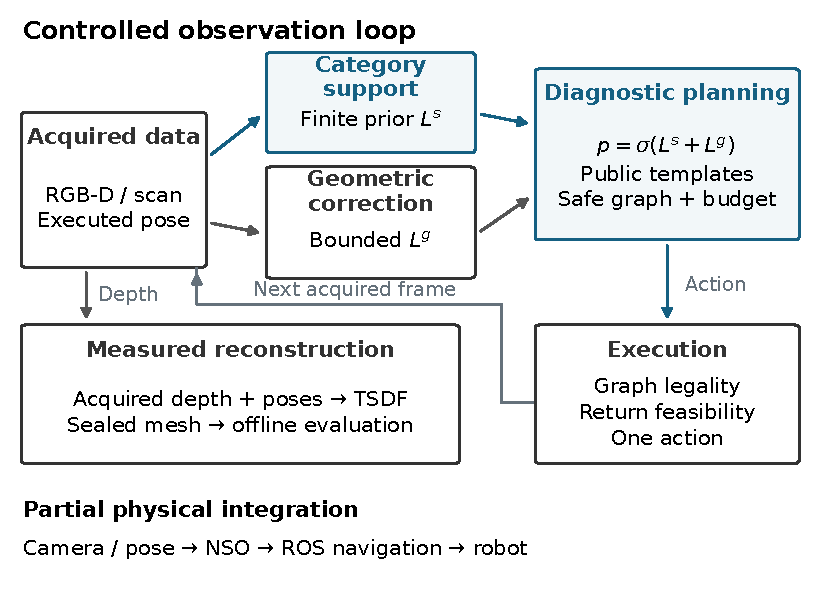
\includegraphics[width=\linewidth,height=.67\textheight,keepaspectratio]{Fig1.pdf}
\caption{Information flow and execution boundary. Category support and acquired geometric evidence update a configuration belief; the planner selects a feasible observation action. Acquired depth separately updates the measured reconstruction. Public predictions score candidate actions and never become fused measurements. The robot interface is an integration path whose current evidence is reported separately in Section~\ref{physical-deployment}}\label{fig:1}
\end{figure}

After action \(t\), the planning state is

\[
x_t=(s_t,b_t,M_{0,t},M_{1,t},p_t,\mathcal V_t),\qquad b_t=B-t.
\]

Here \(s_t\) includes position and heading, \(p_t\) weights configuration 0, and \(\mathcal V_t\) contains measured poses. Each \(M_{h,t}\) records the union of floor samples and surface patches predicted visible from previously observed poses under public template \(h\). These exposure sets support prospective planning; the measured map separately integrates acquired depth. Neither hidden configuration identifiers nor evaluation surfaces enter the state. The common 18-action prefix updates observations and returns to \(s_0\); subsequent actions depend on the resulting belief.

Both hypotheses remain available throughout execution. Category information changes their weights rather than selecting a template as reconstructed truth. The online belief module additionally retains geometric log-support and category-registration history, while each planning call receives their current combined weight. This separates two questions: which configuration the acquired evidence supports, and which affordable observation sequence is valuable under that uncertainty.

\hypertarget{category-support-and-geometric-correction}{%
\subsection{Category support and geometric correction}\label{category-support-and-geometric-correction}}

A category cue must influence early decisions without preventing later contradictory measurements from changing the route. We therefore register finite category support once and combine it with bounded evidence from newly acquired viewpoints. This design allows a cue to establish a preference while preserving both configuration hypotheses.

The category-support function registers a category when its marker occupies at least 16 exact-color pixels at each of two distinct XY positions, without a competing marker in those frames. Registration supplies \(L_t^s=\pm\log9\); repeated detections do not multiply this prior, and conflicting category support clears it. G uses \(L_t^s=0\). Synthetic markers provide a controlled category channel, independently of natural-image recognition performance.

Geometric correction compares acquired depth and scan measurements with both public predictions. Let \(e_{h,t}^{k}\) be the mean residual loss for eligible modality \(k\) under template \(h\), and \(\mathcal K_t\) its valid-modality set. At a newly visited pose,

\[
\begin{aligned}
\delta_t=\operatorname{clip}_{[-6,6]}
\left(\frac{1}{|\mathcal K_t|}\sum_{k\in\mathcal K_t}
\bigl(e_{1,t}^{k}-e_{0,t}^{k}\bigr)\right),\\
L_t^g=\operatorname{clip}_{[-24,24]}(L_{t-1}^g+\delta_t),\qquad
p_t=\sigma(L_t^g+L_t^s).
\end{aligned}
\]

Here \(\sigma(z)=(1+e^{-z})^{-1}\). The increment is zero when no modality qualifies or the pose has already supplied evidence. Residuals use samples where public predictions differ by more than \(10^{-5}\) m. Depth requires eight valid pixels and normalized disparity residual \((57.6/z-57.6/\widehat z_h)/0.25\); scan requires three valid beams and residual \((r-\widehat r_h)/0.02\). Each sample contributes half its squared residual, capped at 12.5. Missing measured returns are ignored; a missing predicted depth return receives the capped loss. Eligible modality means receive equal weight.

These bounded pseudo-likelihoods prevent individual extreme residuals from dominating. They are not calibrated probabilities, and excluding exact repeats does not establish independence between neighboring views. New depth from a repeated pose still contributes to fusion. An incorrect prior remains correctable: for \(L^s>0\), configuration-1 support reaches \(\eta>1/2\) whenever

\[
L_t^g\le-L^s-\operatorname{logit}(\eta).
\]

This threshold is attainable only if sufficient contrary observations occur and the cumulative cap permits it. The finite prior therefore expresses a revisable preference rather than a permanent semantic constraint.

\hypertarget{predictive-value-and-diagnostic-lookahead}{%
\subsection{Predictive value and diagnostic lookahead}\label{predictive-value-and-diagnostic-lookahead}}

A diagnostic view can be valuable because it changes a later route choice, even when its immediate predicted surface gain is small. The planner therefore evaluates future exposure under both configurations and includes one possible diagnostic event within each planning call. Its predicted exposure score guides sensing, while the endpoint score remains a measurement of the reconstructed surface.

For template \(h\), let \(\mathcal F_h\) contain its floor samples, \(\mathcal P_h\) its exterior vertical patches, \(a_u\) the patch area, and \(A_h\) the total exterior vertical area. Writing \(M_h^f\) and \(M_h^s\) for the corresponding exposed subsets gives

\[
\widetilde C_h=\frac{|M_h^f|}{|\mathcal F_h|},\qquad
\widetilde S_h=\min\left(1,\frac{\sum_{u\in M_h^s}a_u}{A_h}\right),\qquad
\widetilde J_h=\widetilde C_h\widetilde S_h.
\]

Thus \(\widetilde S_h\) is an exposed-area fraction, not reconstructed surface F1. The surrogate rewards opportunities to observe missing surfaces but does not model TSDF error or improvements from repeated measurements. Its relation to measured \(J_5\) is tested empirically.

Exposure is accumulated by set union, so viewing an already exposed patch supplies no additional proxy area. Changing direction can still reveal previously occluded patches. Floor samples are those declared by the public planning model, distinct from the finer reachable-cell grid used to measure \(C_{\rm map}\). Consequently, neither component of the surrogate is substituted for an endpoint measurement. Keeping both representations makes the planning assumption explicit: access to additional surface area is a useful, imperfect predictor of reconstructed quality.

Let \(M=(M_0,M_1)\). Stopping requires the complete initial pose and adequate predicted floor exposure under both configurations:

\[
Z(s,M,p)=
\begin{cases}
p\widetilde J_0(M_0)+(1-p)\widetilde J_1(M_1),
&s=s_0,\ \min_h\widetilde C_h(M_h)\ge0.8,\\
-\infty,&\text{otherwise}.
\end{cases}
\]

Diagnostic planning approximates belief-space planning \cite{ref12,ref13} with one future diagnostic event per planning call. Diagnostic candidates are determined from public sensor predictions: treating each template prediction as a hypothetical observation must yield geometric evidence at least \(+\log99\) for configuration 0 and at most \(-\log99\) for configuration 1. Previously measured poses are excluded. This identifies potentially discriminative viewpoints without obtaining their actual observations.

For an anticipated diagnosis of assumed accuracy \(r_d=0.99\), the branch weights and updated planning beliefs are

\[
\begin{aligned}
\lambda_0&=pr_d+(1-p)(1-r_d),\qquad \lambda_1=1-\lambda_0,\\
p^{(0)}&=\frac{pr_d}{\lambda_0},\qquad
p^{(1)}=\frac{p(1-r_d)}{\lambda_1}.
\end{aligned}
\]

Let \(q\in\{0,1\}\) indicate whether this event remains available. Action \(a\) reaches \(s'\), consumes one action, and updates \(M'_h=M_h\cup E_h(s')\), where \(E_h\) is public predicted exposure. The continuation and value recursions are

\[
Q_q(a)=
\begin{cases}
\sum_{y=0}^{1}\lambda_y V_0(s',b-1,M',p^{(y)}),
&q=1,\ s'\text{ diagnostic},\\
V_q(s',b-1,M',p),&\text{otherwise},
\end{cases}
\] \[
V_q(s,b,M,p)=\max\left\{Z(s,M,p),\max_{a\in\mathcal A(s)}Q_q(a)\right\}.
\]

At \(b=0\), only stopping is available. States whose return distance exceeds \(b\) are infeasible, as are diagnostic actions with either infeasible branch. Forecast beliefs remain inside the current calculation. The controller executes only the first selected action, updates belief from acquired measurements, and replans. The category strength 0.9 and forecast accuracy 0.99 are fixed design settings shared across the comparisons, rather than measured classifier or sensor accuracies.

The recursion evaluates complete remaining continuations, rather than immediately visible area alone. Anticipated diagnosis is useful only through the different actions it may enable afterward. Requiring a feasible continuation in both branches prevents a low-weight configuration from being silently discarded to satisfy the return and coverage gates. The approximation limits the number of belief changes within one forecast; it does not limit the number of measured corrections over the executed trajectory. A later call can anticipate another diagnostic event after assimilating the latest frame.

\hypertarget{budgeted-execution-and-reconstruction}{%
\subsection{Budgeted execution and reconstruction}\label{budgeted-execution-and-reconstruction}}

An informative view is useful only if the robot can execute it and still return within budget. The execution layer reserves the shortest graph return cost before each action; the reconstruction layer then integrates only the depth acquired at the executed pose.

The return-feasibility check accepts a legal edge only if

\[
1+d_{\rm return}(s')\le b_t,
\]

where return distance includes restoration of the starting heading. On the fixed graph with unit action costs, this preserves an affordable return path: after each accepted action, \(d_{\rm return}(s_{t+1})\le b_t-1=b_{t+1}\). This certificate concerns graph feasibility; task qualification additionally requires measured coverage, collision-free execution, and actual return.

\par\medskip\noindent\begin{minipage}{\linewidth}
\small\hrule\vspace{0.6em}
\textbf{Algorithm 1. Category-conditioned receding-horizon observation.}

\begin{verbatim}
Input: common graph, templates, budget B, prefix, policy G or S
Initialize belief support, exposures, and visited poses
Repeat:
  Read the initial frame or latest executed-action frame
  Fuse acquired depth exactly once into the measured TSDF
  Register category support and update geometric evidence
  Add current template exposures and record the measured pose
  If collision or budget exhaustion: record termination; exit
  If the shared prefix is unfinished: select its next action
  Otherwise:
    Exclude measured poses from diagnostic candidates
    Solve V1 from the current state and remaining budget
    If infeasible or a resource cap is exceeded: fail; exit
    If stopping is optimal within tolerance: stop; exit
    Select the first maximizing action in fixed graph-edge order
  Check graph legality and the return-budget inequality
  If rejected: record the termination reason; exit
  Execute one action, charge its cost, and obtain the next frame
Output: measured map, trajectory, observations, and stop reason
\end{verbatim}
\vspace{0.4em}\hrule
\end{minipage}\par\medskip


Equal-valued choices use a \(10^{-12}\) tolerance and fixed edge order. The shared Open3D CPU TSDF \cite{ref4,ref11} uses 4 cm voxels and 12 cm truncation; public templates never contribute synthetic depth. Outputs precede independent endpoint evaluation. Incorrect-prior controls exchange category interpretation; the no-correction variant additionally disables measured correction and forecast diagnosis.

For \(N\) poses and exposure bitset lengths \(m_0,m_1\), the cached state count is conservatively bounded by \(K\le3N(B+1)2^{m_0+m_1}\), covering the initial and two post-diagnosis weights. With maximum out-degree \(d\), bitset-update cost \(T_m\), and terminal-evaluation cost \(T_z\), planning costs \(O(K(dT_m+T_z))\), excluding return-distance preprocessing. Each call permits 1.5 million cached states and approximately 20 s; elapsed time is checked every 1024 new states and at selection completion. This finite implementation supports the controlled task, with exponential exposure-state dependence.

\hypertarget{decision-interpretation-and-conditions-for-benefit}{%
\subsection{Decision interpretation and conditions for benefit}\label{decision-interpretation-and-conditions-for-benefit}}

A recorded example connects the recursion to robot behavior. After the common prefix in P00, G assigns both configurations weight 0.5; left/right continuation values of 0.650944 tie. With configuration-1 category support 0.9, S obtains 0.668008/0.711865 and turns right at action 19. A misleading prior can subsequently reverse: geometric evidence of \(-6\) at step 28 gives configuration-1 weight \(1-\sigma(-6+\log9)=0.978178\), followed by a changed action at step 29. These are planning values and belief weights; measured reconstruction outcomes are reported separately.

The underlying tradeoff can be expressed using established belief-based decision principles \cite{ref12,ref13}. Assume two initially equally likely configurations, two return-feasible routes, matched utility \(U_+\), mismatched utility \(U_-\), and \(\Delta=U_+-U_->0\). A category cue has symmetric reliability \(r_c\ge1/2\). Optional geometric diagnosis has symmetric reliability \(r_d\ge1/2\), is conditionally independent given configuration, and costs utility \(\kappa\). Both routes remain feasible afterward. For current belief \(p\), direct choice succeeds with probability \(m=\max(p,1-p)\); optimal choice after diagnosis succeeds with probability \(\max(m,r_d)\). Its net value is

\[
\Delta\max(0,r_d-m)-\kappa.
\]

G benefits from diagnosis when \(\kappa<(r_d-1/2)\Delta\), whereas a category-conditioned decision requires \(\kappa<(r_d-r_c)_+\Delta\), with \(\kappa\ge0\). An informative cue can therefore avoid a diagnostic detour while preserving a useful observation direction. Its benefit disappears when geometry already resolves the choice or route utilities coincide. When \(r_d\ge r_c\) and diagnosis is free, both policies can attain the same expected directional utility; a free but less reliable diagnosis need not remove the category advantage. These analytical reliabilities are assumptions distinct from implementation settings. The argument identifies conditions for improved allocation; it does not guarantee better measured reconstruction under the exposure surrogate.

The practical consequence is a conditional experimental prediction: a category cue should matter when it changes a consequential route ranking before equivalent geometric evidence is affordable. If geometry and category already favor the same route, identical actions and quality are expected. Tests therefore examine action changes, acquired surfaces, and measured quality together, rather than interpreting stronger belief alone as a mapping improvement.

\hypertarget{experiments-and-results}{%
\section{Experiments and Results}\label{experiments-and-results}}

The controlled experiments test category-conditioned observation at matched coverage, geometric correction, and sensitivity to budget and changed backgrounds. Sections~\ref{joint-exploration} and~\ref{physical-deployment} evaluate unknown-exploration and physical deployment separately.

\hypertarget{experimental-setup-and-matched-comparisons}{%
\subsection{Experimental setup and matched comparisons}\label{experimental-setup-and-matched-comparisons}}

The simulator supplies 96\ensuremath{\times}72 depth images over a 4 m range and a 360\ensuremath{^{\circ}} planar scan with 180 beams over 8 m. Poses are exact. Depth noise has a standard deviation of 0.25 pixels in reference disparity; no additional random scan noise is applied. The experiments isolate planning under controlled observations rather than reproduce physical sensor errors.

The evaluator derives the start-reachable safe-cell set \(\mathcal R\) using a 0.2 m grid and 0.2 m robot radius. It contains 588 cells in P00 and 668 in P01. A nonunknown cell counts as observed, including one marked occupied, so coverage is not occupancy-classification accuracy. Ground truth is used after prediction sealing, not to supply runtime measurements.

Surface precision and recall follow distance-threshold comparison \cite{ref14}. Precision queries the reference from sampled predicted surfaces; recall queries the prediction from fixed exterior vertical reference surfaces. The prediction is cropped to the common bounding box of both templates with a 0.20 m margin, and the known ground is removed. Thus, errors outside this region do not enter precision. No registration or hole filling is applied. Thresholds are fixed at 2, 5, and 10 cm, with 5 cm primary; empty predictions receive zero quality. Coverage, precision, recall, and task qualification accompany the product to avoid hiding its components.

Confirmation freezes the controller and uses a held-out noise seed on two previously seen parent layouts, each with two configurations: eight runs and four G/S pairs. The layout-level units are the two parent layouts. Two configurations per layout and repeated noise realizations are paired conditions, not independent evidence of category-level generalization. The policies differ as follows: G has no category support; S uses the designated correct cue; X reverses the category interpretation; and Xnf uses the same reversed interpretation while disabling measured correction and future diagnostic anticipation. The development X/Xnf contrast therefore evaluates the bundled correction policy. Replays and alternative thresholds reuse these trajectories; they do not increase the number of independent layouts or trials. The principal G control retains the diagnostic views and revisiting available to S; Xnf deliberately disables measured correction and anticipated diagnosis.

For each matched condition we report the absolute score difference, \(\Delta J_5=J_{5,S}-J_{5,G}\). A relative mean change is \(100(\overline J_{5,S}/\overline J_{5,G}-1)\), rather than an average of per-condition percentages. Qualification is reported over all declared attempts; endpoint means include only the explicitly qualified groups.

The recorded software is Python 3.12.3, NumPy 1.26.4, SciPy 1.11.4, and Open3D 0.19.0, with one OpenMP, OpenBLAS, and MKL thread. No GPU is required. Figures use actual recorded actions and measured meshes except the explicitly schematic architecture diagram.



\hypertarget{surface-reconstruction-at-matched-coverage}{%
\subsection{Surface reconstruction at matched coverage}\label{surface-reconstruction-at-matched-coverage}}

Across the four confirmation conditions in Table 2, mean \(J_5\) increases from 0.702576 to 0.745881, a relative improvement of 6.1638\%. Every run uses 42 actions, avoids collision, and returns exactly. Mean coverage is identical at 0.952544; mean surface F1 increases from 0.737490 to 0.782951. This decomposition attributes the observed joint-score gain to surface reconstruction at matched planar coverage.

\begin{table}[!htbp]
\caption{Complete confirmation pairs; relative change compares policy means}\label{tab:2}
\small\renewcommand{\arraystretch}{1.12}\setlength{\tabcolsep}{3pt}
\setlength{\JournalTableWidth}{\dimexpr\linewidth-6\tabcolsep\relax}
\begin{tabular}{@{}>{\raggedright\arraybackslash}p{0.32\JournalTableWidth} >{\raggedright\arraybackslash}p{0.22\JournalTableWidth} >{\raggedright\arraybackslash}p{0.22\JournalTableWidth} >{\raggedright\arraybackslash}p{0.24\JournalTableWidth}@{}}
\toprule
Layout/configuration & G: \(J_5\) & S: \(J_5\) & S\ensuremath{-}G \\
\midrule
P00/h0 & 0.772200 & 0.772200 & 0 \\
P00/h1 & 0.672703 & 0.760456 & +0.087753 \\
P01/h0 & 0.727281 & 0.727281 & 0 \\
P01/h1 & 0.638118 & 0.723586 & +0.085468 \\
Mean & 0.702576 & 0.745881 & +0.043305 \\
\bottomrule
\end{tabular}
\end{table}

In both h1 cases, category conditioning changes the first autonomous turn. The resulting surface recall rises from 0.5958 to 0.7249 in P00 and from 0.5555 to 0.6845 in P01. Both h0 pairs follow identical trajectories. The relative mean gains at 2 and 10 cm are 5.5040\% and 6.2110\%, respectively. These descriptive sensitivities do not establish statistical significance across unseen layouts. The primary outcome pattern is two wins, two ties, and no losses across four configuration pairs; the two ties are exact trajectory and metric matches. We therefore report every pair and the absolute mean difference of 0.043305 alongside the relative mean change. No confidence interval treating configurations, seeds, frames, or checkpoints as independent layouts is used.



Retained endpoint meshes show the recovered side structures using matched cameras and scales. P00/h1 needs 28 m and 14 turns for G versus 26 m and 16 turns for S; P01/h1 uses 28 m and 14 turns for both. Every run acquires the same number of frames. The effect therefore depends on allocating observations differently, rather than increasing sensing or travel.



\hypertarget{geometric-correction-and-reconstruction-progress}{%
\subsection{Geometric correction and reconstruction progress}\label{geometric-correction-and-reconstruction-progress}}

The P00 development timeline connects the decision example in Section 4.5 to acquired evidence. Category support changes the first autonomous observation direction at action 19, while subsequent geometric measurements can reverse the influence of an incorrect cue.

With the incorrect cue, X initially assigns configuration 1 a weight of 0.1. At step 28, 1092 informative depth pixels provide sufficient contrary evidence to raise this weight to 0.978178. X then moves forward at action 29, while Xnf turns right. Across the two development configurations, X improves mean \(J_5\) over Xnf from 0.655065 to 0.672254, or 2.6241\%. Because Xnf also removes anticipated diagnosis, this is not an isolated posterior-update ablation. At the stricter 2 cm threshold, the h1 difference is \ensuremath{-}0.00216, indicating that correction does not improve every surface-scale measure.



We further reintegrate the eight saved confirmation trajectories at 18, 24, 30, 36, and 42 paid actions: 40 measured checkpoints, with unchanged observations, poses, fusion settings, and evaluator. All 16 previously available prefix/endpoint checkpoints reproduce their original metrics exactly. Coverage matches within every pair at every checkpoint and reaches its endpoint value by action 30. Later differences mainly accompany increased surface recall and F1. P00/h1 is still slightly worse for S at action 24 (\ensuremath{-}0.000819), then positive at 30, 36, and 42; P01/h1 is already positive at 24. Both h0 pairs remain tied. Intermediate states may not satisfy return or coverage requirements and are not successful terminal trials.



\hypertarget{sensitivity-to-budget-noise-and-facility-geometry}{%
\subsection{Sensitivity to budget, noise, and facility geometry}\label{sensitivity-to-budget-noise-and-facility-geometry}}

The fixed extension declares 128 trials. Original P00/P01, two configurations, budgets 30/42/54, two noise seeds, and four policies define 96 trials. Two same-family variants at budget 42 add 32: one P00 rib shifts 0.25 m, while three P01 ribs lower their upper boundary from 1.80 to 1.35 m. Transformations apply consistently to both public hypotheses, sensed geometry, and reference surfaces. The safe graph, prefix, controller, and prior settings remain unchanged. These variants test nearby geometry, not unseen natural equipment categories.

All 128 tasks are attempted once: 96 qualify and 32 fail at budget 30 after the common prefix. The controller cannot find a return plan meeting its predicted 80\% coverage gate under both templates. This is a planning-constraint boundary, not universal physical impossibility. Failure maps remain separate from successful endpoint means.

\begin{table}[!htbp]
\caption{Complete extension groups. Each row declares 32 trials; qualified rows contain eight per policy}\label{tab:4}
\small\renewcommand{\arraystretch}{1.12}\setlength{\tabcolsep}{3pt}
\setlength{\JournalTableWidth}{\dimexpr\linewidth-10\tabcolsep\relax}
\begin{tabular}{@{}>{\raggedright\arraybackslash}p{0.26\JournalTableWidth} >{\raggedright\arraybackslash}p{0.148\JournalTableWidth} >{\raggedright\arraybackslash}p{0.148\JournalTableWidth} >{\raggedright\arraybackslash}p{0.148\JournalTableWidth} >{\raggedright\arraybackslash}p{0.148\JournalTableWidth} >{\raggedright\arraybackslash}p{0.148\JournalTableWidth}@{}}
\toprule
Condition/budget & Qualified & G: \(J_5\) & S: \(J_5\) & S/G change & S/G win / tie / loss \\
\midrule
Original/30 & 0/32 & --- & --- & --- & --- \\
Original/42 & 32/32 & 0.702648 & 0.746567 & +6.2505\% & 4 / 4 / 0 \\
Original/54 & 32/32 & 0.926298 & 0.919819 & \ensuremath{-}0.6995\% & 0 / 4 / 4 \\
Variants/42 & 32/32 & 0.704562 & 0.734357 & +4.2289\% & 4 / 4 / 0 \\
\bottomrule
\end{tabular}
\end{table}

The three qualified groups each contain eight G/S pairs, including two noise seeds per geometry/configuration condition. The bundled X/Xnf correction contrast improves its group mean by 1.7328\%, 2.5163\%, and 1.7016\% for original/42, original/54, and variants/42, respectively. These are correction-policy contrasts, not isolated module estimates.

At budget 42, improvements occur in the h1 configurations of both the original and variant layouts, while the h0 routes remain unchanged. At budget 54, the mean difference reverses to \ensuremath{-}0.6995\%, with lower scores in four conditions and unchanged scores in the other four. Coverage reaches 1.0 for both policies; G/S recall is 0.985764/0.983826 and precision 0.873764/0.863789. The negative difference mainly accompanies lower precision, exposing a gap between template exposure and measured reconstruction. This decomposition does not independently identify a fusion-error cause. X also exceeds G/S at this budget, so a correct prior does not guarantee the best measured endpoint under the finite-lookahead surrogate.

The two variants individually improve S/G by 5.0337\% and 3.3974\%. At 2/5/10 cm, original-layout improvements at budget 42 are 5.4991\%/6.2505\%/6.3063\%, whereas budget-54 differences are \ensuremath{-}1.2217\%/\ensuremath{-}0.6995\%/\ensuremath{-}0.2866\%. The reversal is therefore not created by selecting the primary threshold. Noise repeats describe the same geometry and are not additional independent layouts.



\hypertarget{transfer-to-changed-background-layouts}{%
\subsection{Transfer to changed background layouts}\label{transfer-to-changed-background-layouts}}

A final protocol fixes two additional layouts before observing results: a side column removes one right-aisle navigation center, while a rear partition interrupts direct rear passage. Both retain the P00 facility family and public templates. The controller, category mapping, sensor noise rule, fusion, evaluation region, 18-action common prefix, and 42-action budget remain unchanged. All legal safe-grid centers are retained; each new layout has 23 centers and 92 oriented poses. The noise seed is the original confirmation seed, so this test adds two background-layout units, not new noise replicates or unseen facility categories. Each layout uses both configurations and G/S, giving eight tasks and four pairs.

All eight tasks complete 42 paid actions and 43 acquired frames, avoid collision, and return to the full initial pose. Table \ref{tab:5} reports every paired endpoint. Mean coverage is identical at 0.934732; mean precision increases from 0.864441 to 0.870224, recall from 0.672455 to 0.704742, and surface F1 from 0.754450 to 0.777445. Mean joint quality increases from 0.705188 to 0.726215, or 2.9818\%. The gain is concentrated in the rear-partition h1 condition; the other three conditions retain the same trajectories and endpoint quality. Relative differences at 2 and 10 cm are 2.8176\% and 3.1200\%. These are descriptive paired results from two new layouts; configurations do not increase the number of independent layout units.

\begin{table}[!htbp]
\caption{Changed-background results at 5 cm for all four paired conditions. Coverage is equal within each pair; all eight tasks qualify}\label{tab:5}
\small\renewcommand{\arraystretch}{1.12}\setlength{\tabcolsep}{3pt}
\setlength{\JournalTableWidth}{\dimexpr\linewidth-10\tabcolsep\relax}
\begin{tabular}{@{}>{\raggedright\arraybackslash}p{0.26\JournalTableWidth} >{\raggedright\arraybackslash}p{0.148\JournalTableWidth} >{\raggedright\arraybackslash}p{0.148\JournalTableWidth} >{\raggedright\arraybackslash}p{0.148\JournalTableWidth} >{\raggedright\arraybackslash}p{0.148\JournalTableWidth} >{\raggedright\arraybackslash}p{0.148\JournalTableWidth}@{}}
\toprule
Layout / config. & Coverage & G F1 & S F1 & G joint & S joint \\
\midrule
Side column / h0 & 0.954145 & 0.806490 & 0.806490 & 0.769508 & 0.769508 \\
Side column / h1 & 0.955908 & 0.702575 & 0.702575 & 0.671597 & 0.671597 \\
Rear partition / h0 & 0.914439 & 0.806490 & 0.806490 & 0.737485 & 0.737485 \\
Rear partition / h1 & 0.914439 & 0.702246 & 0.794224 & 0.642160 & 0.726269 \\
Mean & 0.934732 & 0.754450 & 0.777445 & 0.705188 & 0.726215 \\
\bottomrule
\end{tabular}
\end{table}

The retained trajectories show the effect's dependence on the available observation routes. In the side-column layout, both initial directions are return-feasible. Category information changes their predicted values but preserves their ordering, so both planners select the same route. In the rear-partition h1 condition, G assigns nearly equal values to the two directions and selects left through its fixed tie rule, whereas S selects right. Up to step 18 their acquired nonsemantic histories and geometric support are identical. The category-conditioned decision changes action 19 and improves endpoint surface recall from 0.595795 to 0.724945. In this condition, \(J_5\) rises from 0.642160 to 0.726269, a relative improvement of 13.10\%, at unchanged coverage and action count. This is a complete-route effect: the subsequent measurements differ, so the endpoint gain is not attributed to a single frame.



G/S mean travel is 27.0/26.5 m, with 15.0/15.5 turns. Single-thread planning wall time averages 0.0474/0.0484 s per task on an Intel Xeon processor (Sapphire Rapids); complete task times, including sensing, fusion and evaluation, range from 5.0 to 5.8 s. Timing is descriptive for this four-logical-CPU host, not a real-time or cross-hardware benchmark. The controller and all evaluation settings remain fixed throughout this background-layout comparison.

\hypertarget{evaluation-boundaries}{%
\subsection{Evaluation boundaries}\label{evaluation-boundaries}}

We retain three distinct experimental units: parent layouts, paired configuration conditions within a layout, and repeated measurements along an existing trajectory. The 40 reconstruction checkpoints belong to eight trajectories; the 128 attempts include repeated noise conditions and four policies. A separately retained 36-attempt multi-instance study compares controller versions. It includes nine shared/fixed-prior ties and adverse category comparisons, with 35 original evaluation-pipeline completions and one separately corrected numerical evaluation; it supplies no cross-instance-sharing benefit. Adding these counts does not produce a single sample size. Endpoint summaries are accompanied by qualification counts, and failed tasks remain in the attempted-task denominator. The present small number of independent layouts supports descriptive paired comparisons, not a population-level superiority claim.


\section{Joint Unknown-Space Exploration Diagnostic}\label{joint-exploration}

Unknown-space exploration remains the broader system objective. A separate 24-trajectory diagnostic starts from a simulated RGB-D/scan packet at 61.50\% reachable-cell coverage, using exact poses and a 0.2 m grid/radius. It compares original V10.3.1 G/S, exploration\_joint\_v1 C/G/S and a local observed-frontier implementation at 48/96-action limits in two related arrangements of one Q0 scene. The joint variant restricts coverage gain to unknown support, diversifies candidates and replans invalidated macro-actions. These declared policy changes distinguish it from the supplied-graph mechanism. All runs return without simulated collision; east/96 C uses 94 actions and the others exhaust their limits. Supplementary Tables S1--S2 retain every outcome.

Three of four G/S conditions tie within each version. In west/96, original S recovers less new reference-visible surface than G (111.44/114.11 m$^2$), while joint S recovers more (118.52/109.51 m$^2$). Joint G/S reach 90/95/99\% coverage at identical actions 18/24/29, with surface histories diverging after 99.55\% coverage. At budget 48, frontier reaches 95\% coverage earlier and gains more observed area, while joint C/G/S recover more surface. The frontier adapter permanently returns after rejection, unlike NSO replanning; common execution protection does not imply equivalent policy contracts.

A post-hoc doubled geometric-prior control exactly reproduces the improved S trajectory in a related two-room case. A separate paid-41 west/96 intervention isolates a ranking unavailable to uniform nonnegative prior reweighting on that saved set, yet gains surface and loses terminal F1 against G. A further synthetic parent fixed before execution yields 11.72 m$^2$ more new surface and 0.04856 higher F1 for S than G/X over complete 96-action routes, but all saved S decisions admit a common geometric-prior weight (supplementary Table S3). These related diagnostics establish conditional allocation effects, with general early-coverage efficiency and category-specific attribution unresolved.

\section{Physical Deployment Pilot}\label{physical-deployment}
The physical deployment is a declared joint-exploration variant, distinct from the supplied-graph, two-template controlled study. It uses exploration\_joint\_v1 derived from v10\_3\_1, with revised joint unknown-coverage and measured-surface candidate generation, real-scene semantics, measured sensor-range and 3 m extent adapters (rather than the original 2.2 m applicability cap), default CSM keyframes, measured CAN controller velocity and fixed SE2 alignment. The camera had been relocated without recalibrating its earlier extrinsics; its earlier self-mask was disabled. The navigation map retained prior observations in the first episode.

One S40 episode completed 40 paid actions and 40 arrivals, returned to its grid anchor, and acquired 41 frames over 7.394 m of CAN-estimated travel and 542.444 s. Its observed-area proxy increased from 72.08 to 128.28 m$^2$, while its fixed old-surface quality proxy decreased from 0.213760 to 0.199107. These are internal proxies, without an independent map or surface-accuracy reference. All 12 recorded planning states gave equal G and S scores for shared candidates; only two had multiple candidates. This does not constitute a separate G trial.

\subsection{Fresh-map ordered C/S physical pilot}

A subsequent pilot executed coverage-only C followed by joint S in the same physical scene. Each arm used a fresh, separately supervised stock gmapping instance and a new policy session, with the same 40-action budget, 600 s limit, circular footprint, candidates, return rule, sensing configuration and execution protection. Only score mode differed within the policy configuration; C retained the same candidate generator and sensor modalities. CSM odometry and the display TSDF remained continuous. The actual bootstraps differed by 0.0701 m and 0.0672 rad, and their initial navigation-known masks differed in 205 cells (8.20 m$^2$) on the common 0.2 m planning grid. This is an approximate starting-condition comparison, not identical-input pairing.

\begin{table}[!htbp]
\caption{One ordered physical C/S pilot with fresh navigation maps; failures remain included}\label{tab:physical-pair}
\small\renewcommand{\arraystretch}{1.12}\setlength{\tabcolsep}{3pt}
\begin{tabular}{@{}>{\raggedright\arraybackslash}p{.18\linewidth}p{.12\linewidth}p{.18\linewidth}p{.17\linewidth}p{.23\linewidth}@{}}
\toprule
Arm and termination & Paid / obs. & CAN / time & Internal area (m$^2$) & Own-support old-quality \\
\midrule
C: budget exhausted, returned & 40 / 41 & 6.741 m /\newline 558.214 s & 66.40 $\to$ 123.44 & 0.249536 $\to$ 0.190989 (270 points) \\
S: method failure, no return & 32 / 33 & 5.233 m /\newline 451.992 s & 65.32 $\to$ 122.00 & 0.234949 $\to$ 0.299275 (290 points) \\
\bottomrule
\end{tabular}
\end{table}



\begin{figure}[!htbp]
\centering
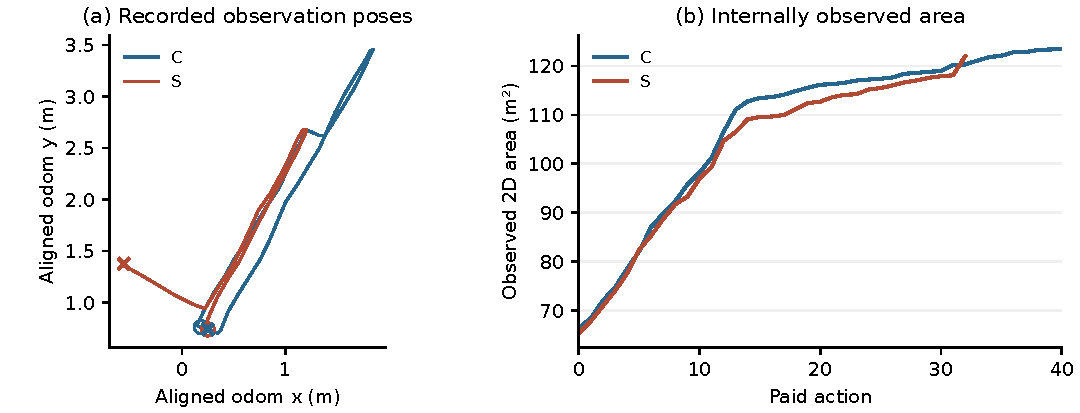
\includegraphics[width=\linewidth]{PhysicalPair_C_S_20261107.pdf}
\caption{Recorded aligned-odometry poses and internal observed-area proxy in the ordered C/S pilot. S stops after action 32; no continuation is inferred. The two episodes use different initial measurements and provide no independent accuracy reference.}
\label{fig:physical-pair}
\end{figure}

C completed its budget and returned to the discrete anchor. S stopped after its 32nd accepted action when the existing circular-footprint check reported \texttt{current\_footprint\_not\_known\_safe}; it did not return. This was an original method check, not a newly introduced policy gate. CAN feedback was zero after both runs. Unequal completed actions, the failed S return, and different initial information prevent an efficiency ranking or a causal policy-benefit claim. Quality is reported separately on each arm's own fixed bootstrap support, whose identities differ; the C decrease and S increase are not a matched reconstruction-accuracy comparison. This C/S objective ablation does not isolate a semantic S/G effect.

At paid action 12, both runs replanned after the original next-footprint check; at each run's own state, C and S selected the same candidate, while the maps differed across runs. At S action 31, frozen-state C had no positive candidate whereas G and S selected the same positive candidate. These recorded counterfactuals are not additional physical trials, and G/S ties do not establish a semantic decision effect.

A mapper-only replay of the retained S observations reproduced the final belief: a measured 0.504 m laser return inserted a nearby occupied cell before depth fusion, while the input navigation grid alone still passed the footprint check. This identifies the recorded fusion source, not the physical object or a verified noise or localization cause.


% Single insertion point for new physical evidence. Replace only from verified terminal records.
\subsection{Calibrated 24-action integration run}

After revising the camera extrinsics, a later S24 integration episode completed 24 paid actions, 24 verified arrivals and 25 observations, returning to its discrete anchor over 3.591 m of CAN-estimated travel and 368.847 s. This episode used a different sensor calibration and map state from the earlier C/S pilot and is not a matched continuation or policy comparison. All six newly recorded planning states gave equal G/S candidate scores and zero incremental aperture contribution, so they show no semantic selection effect.

After the run, the operator reported that localization had drifted during the preceding manual relocation to the test area. The drift onset was not established, so the map at S24 initialization may already have been affected. Discrete-anchor acceptance and measured travel therefore support bounded execution integration, not independent localization accuracy, comparative exploration efficiency or reconstruction accuracy. The internal area proxy (180.12 to 256.60 m$^2$) is not treated as verified newly discovered physical area. A subsequent mapping reset starts a new epoch; its observations cannot be pooled with this episode as a shared initial map.

\subsection{Calibrated fresh-map C/S comparison}

A new ordered C/S pilot used independently restarted stock gmapping maps and fresh acquired initial packets in the reset localization epoch. Both arms retained the same 40-action allowance, 600 s external limit, circular footprint, candidate generator, return rules, sensor configuration and ROS/hardware protection. The score mode was the policy difference; this remains a coverage-only versus joint-objective comparison, not a semantic-only ablation. The planning transform was identical and anchored at the actual C start. Initial odometry differed by 0.06695 m and $-0.06259$ rad, while the initial navigation-known masks differed in 430 cells (17.20 m$^2$) on the common grid. Similar initial area therefore does not imply identical initial information.

\begin{table}[!htbp]
\caption{One further ordered C/S pilot after calibration and map reset. Both arms have a 40-action/600 s allowance; actual exposure and return differ. Internal quality uses a separate fixed bootstrap support in each arm.}\label{tab:physical-pair-calibrated}
\small\renewcommand{\arraystretch}{1.12}\setlength{\tabcolsep}{3pt}
\begin{tabular}{@{}>{\raggedright\arraybackslash}p{.18\linewidth}p{.12\linewidth}p{.18\linewidth}p{.17\linewidth}p{.23\linewidth}@{}}
\toprule
Arm and termination & Paid / obs. & CAN / time & Internal area (m$^2$) & Own-support old-quality \\
\midrule
C: no positive option at anchor, returned & 24 / 25 & 3.738 m /\newline 342.345 s & 65.24 $\to$ 98.52 & 0.165048 $\to$ 0.277736 (479 points) \\
S: anchor-footprint failure, no return & 13 / 14 & 1.857 m /\newline 184.862 s & 65.32 $\to$ 88.88 & 0.193484 $\to$ 0.180111 (437 points) \\
\bottomrule
\end{tabular}
\end{table}

C completed 24 verified arrivals and stopped normally under the original rule that stops when no positive option remains at the anchor. S completed 13 verified arrivals, then failed the original check requiring the anchor footprint to remain known safe without returning. Neither endpoint was an external timeout or interruption, and both recorded zero CAN feedback after closing. At S action 10, the original next-footprint rejection triggered replanning; C and S would select different candidates at that saved state, while G and S were tied. Across both episodes, all five candidate-bearing planning states gave equal G/S scores; the terminal S state had no candidates. These are within-state diagnostics, not separately executed alternatives.

The shorter failed S route supplies no efficiency benefit. Unequal completed exposure, different initial measurements and distinct fixed surface supports prevent a matched endpoint-quality or causal policy ranking. This is one ordered pair in one physical scene, with no independent localization, map or surface-accuracy reference. No return override or replacement policy was introduced after the anchor check failed.


\hypertarget{discussion}{%
\section{Discussion}\label{discussion}}

\hypertarget{when-category-information-has-decision-value}{%
\subsection{When category information has decision value}\label{when-category-information-has-decision-value}}

The results connect three events: an early category cue changes a feasible observation direction, the resulting route acquires different surfaces, and those measurements improve reconstructed surface recall at matched coverage. This chain is visible in both reference h1 configurations and in the rear-partition h1 condition. When category information changes scores without changing their ordering, as in the side-column layout, the resulting trajectory and quality remain unchanged. These cases explain why semantic availability alone is insufficient: the cue must alter an executable decision with a useful downstream consequence.

Budget determines the opportunity for that consequence. At 42 actions, the original and same-family geometry groups show positive mean gains. At 30 actions, the planner cannot meet its predicted coverage and return constraints. At 54 actions, both policies reach complete planar coverage, while S has slightly lower surface precision and joint quality. The decision analysis assumes meaningful directional utilities; the implemented template-exposure surrogate does not model all depth-fusion errors. Its mismatch with measured surface quality is therefore a concrete target for improvement, without treating the observed reversal as evidence for a particular unmeasured sensor-error cause.

\hypertarget{scope-of-the-evidence-and-extensions}{%
\subsection{Scope of the evidence and extensions}\label{scope-of-the-evidence-and-extensions}}

The controlled local method uses public configuration templates, a supplied safe graph, exact poses, and synthetic category cues. These assumptions isolate the planning value of category information. The separate joint-exploration diagnostic starts from acquired simulated data, but its related layouts and exact poses do not establish general exploration efficiency. A natural semantic frontend is connected in the separately declared deployment variant, but matched semantic benefit and estimated-pose accuracy remain unvalidated. The background test adds two layouts within the P00 facility family. Configuration pairs, noise repeats, and reconstruction checkpoints do not constitute additional independent layout samples. The results are descriptive evidence of the tested mechanism, rather than a statistical claim of general superiority. SWAP-I and VISTA-I adapt selected mechanisms to a common CPU setting; the TARE runs demonstrate integration feasibility. These comparisons do not rank the corresponding complete original systems.

Section~\ref{physical-deployment} reports actual ROS 1 deployment observations. The comparative reconstruction-quality results remain simulated, while the physical records include completed joint-exploration episodes and two ordered fresh-map C/S pilots with incomplete S returns; semantic transfer remains unverified. Industrial relevance currently concerns observation after workspace reconfiguration with a static environment during acquisition. Mapping drift in the later physical integration run further limits interpretation of measured area and return acceptance. Independent localization and surface references are needed for accuracy claims. Continuous map maintenance and dynamic obstacle avoidance are outside this evaluation.

\hypertarget{conclusion}{%
\section{Conclusion}\label{conclusion}}

This study examines how a correctable category prior affects active observation under a fixed sensing and return budget. The policy uses category information to rank future routes, revises that preference using acquired geometry, and reconstructs surfaces only from measured depth. Against a matched active geometric control, the reference and changed-background comparisons improve mean joint coverage--surface quality by 6.16\% and 2.98\% at unchanged coverage. The paired patterns are two wins/two ties and one win/three ties. The practical finding is conditional: the cue is useful when it changes an affordable observation route whose measurements recover additional surface geometry.

The current evidence is bounded by public templates, a supplied graph, exact simulated poses, and a synthetic category channel. Low-budget failures, larger-budget reversals, and neutral or adverse multi-instance outcomes show that the exposure surrogate and category cue do not ensure better reconstruction. Existing correction controls bundle two mechanisms, and physical records do not establish a matched semantic benefit. The joint-exploration simulations retain unknown-space discovery as an explicit objective, but show late semantic surface effects, geometric-weight ambiguity and no consistent early-coverage gain. The next validation priorities are independently specified exploration layouts, crossed correction/diagnosis controls, and repeated physical comparisons with reliable localization and matched initialization.

\hypertarget{reproducibility-and-data}{%
\section{Reproducibility and Data}\label{reproducibility-and-data}}

For code navigation, category support, diagnostic planning, the return-feasibility check, and geometric correction correspond to the historical interface labels OV-SDF, STGHP, RPN-UQ, and IGCR, respectively. The manuscript uses functional names consistently; these labels do not identify separate learned networks.

The full evidence, negative outcomes, frozen source and policy replay are indexed in the accompanying supplement. Canonical robot inputs contain derived sensor arrays and cached labels; they do not independently reproduce detection. Raw physical packets remain separately retained. The physical episodes summarized here and their repeated observations are not independent scene replications. The 24-trajectory unknown-exploration matrix, related two-room diagnostic and post-hoc continuations remain distinct from the controlled two-template pairs.

\begin{thebibliography}{99}
\bibitem{ref9} World Economic Forum. Physical AI: Powering the New Age of Industrial Operations. White paper, 2025-09-04. \href{https://www.weforum.org/publications/physical-ai-powering-the-new-age-of-industrial-operations/}{Official white paper}.

\bibitem{ref10} Placed J. A., Strader J., Carrillo H., Atanasov N., Indelman V., Carlone L., Castellanos J. A. A Survey on Active Simultaneous Localization and Mapping: State of the Art and New Frontiers. IEEE Transactions on Robotics, 2023. \url{https://doi.org/10.1109/TRO.2023.3248510}.

\bibitem{ref5} Cao C., Zhu H., Choset H., Zhang J. TARE: A Hierarchical Framework for Efficiently Exploring Complex 3D Environments. RSS, 2021. \url{https://doi.org/10.15607/RSS.2021.XVII.018}.

\bibitem{ref1} Chaplot D. S., Gandhi D., Gupta S., Gupta A., Salakhutdinov R. Learning to Explore using Active Neural SLAM. ICLR, 2020. Author manuscript: \url{https://doi.org/10.48550/arXiv.2004.05155}.

\bibitem{ref6} Chen X., Li Q., Wang T., Xue T., Pang J. GenNBV: Generalizable Next-Best-View Policy for Active 3D Reconstruction. CVPR, 2024:16436--16445. \url{https://doi.org/10.1109/CVPR52733.2024.01555}.

\bibitem{ref4} Zhou Q.-Y., Park J., Koltun V. Open3D: A Modern Library for 3D Data Processing. arXiv:1801.09847, 2018. \url{https://doi.org/10.48550/arXiv.1801.09847}.

\bibitem{ref11} Curless B., Levoy M. A Volumetric Method for Building Complex Models from Range Images. Proceedings of SIGGRAPH, 1996:303--312. \url{https://doi.org/10.1145/237170.237269}.

\bibitem{ref2} Dharmadhikari M., Alexis K. Semantics-aware Exploration and Inspection Path Planning. ICRA, 2023. \url{https://doi.org/10.1109/ICRA48891.2023.10160469}.

\bibitem{ref7} Dharmadhikari M., Alexis K. Semantics-Aware Predictive Inspection Path Planning. IEEE Transactions on Field Robotics, 2025. \url{https://doi.org/10.1109/TFR.2025.3578402}.

\bibitem{ref3} Nagami K., Chen T., Yu J., Shorinwa O., Adang M., Dougherty C., Cristofalo E., Schwager M. VISTA: Open-Vocabulary, Task-Relevant Robot Exploration With Online Semantic Gaussian Splatting. IEEE Robotics and Automation Letters, 11(3):3150--3157, 2026. \url{https://doi.org/10.1109/LRA.2026.3653276}.

\bibitem{ref8} Chen L., Zhan H., Yin H., Xu Y., Mordohai P. Understanding while Exploring: Semantics-driven Active Mapping. Advances in Neural Information Processing Systems, 38, 2025. \url{https://doi.org/10.52202/085713-1113}.

\bibitem{ref12} Kaelbling L. P., Littman M. L., Cassandra A. R. Planning and Acting in Partially Observable Stochastic Domains. Artificial Intelligence, 101(1--2):99--134, 1998. \url{https://doi.org/10.1016/S0004-3702(98)00023-X}.

\bibitem{ref13} Hollinger G. A., Sukhatme G. S. Sampling-based Robotic Information Gathering Algorithms. The International Journal of Robotics Research, 33(9):1271--1287, 2014. \url{https://doi.org/10.1177/0278364914533443}.

\bibitem{ref14} Knapitsch A., Park J., Zhou Q.-Y., Koltun V. Tanks and Temples: Benchmarking Large-Scale Scene Reconstruction. ACM Transactions on Graphics, 36(4), 2017. \url{https://doi.org/10.1145/3072959.3073599}.
\end{thebibliography}

\section*{Statements and Declarations}
\subsection*{Funding}
\textit{} \underline{\hspace{5cm}}
\subsection*{Competing interests}
\textit{} \underline{\hspace{5cm}}
\subsection*{Author contributions}
\textit{} \underline{\hspace{5cm}}
\subsection*{Data and code availability}
See the Reproducibility and Data section and accompanying supplement.
The final public version identifier and any access restrictions require author confirmation.
\subsection*{AI assistance disclosure: draft for author confirmation}
OpenAI Codex assisted with manuscript organization and revision and with developing
experiment, analysis, and plotting code. Tool/model versions, the extent of assistance,
and the authors' verification and responsibility statement must be completed before submission.
This draft disclosure does not assert that the authors have already approved the manuscript.

\end{document}
